% Template for ICIP-2022 paper; to be used with:
%          spconf.sty  - ICASSP/ICIP LaTeX style file, and
%          IEEEbib.bst - IEEE bibliography style file.
% --------------------------------------------------------------------------
\documentclass{article}
\usepackage{spconf,amsmath,graphicx}

% Example definitions.
% --------------------
\def\x{{\mathbf x}}
\def\L{{\cal L}}

% Title.
% ------
\title{Learned image compression}
%
% Single address.
% ---------------
\name{Juha Ylikoski, Teemu Eerola, Nardos Estifanos}
\address{juha.ylikoski@tuni.fi, teemu.eerola@tuni.fi, nardos.estifanos@tuni.fi}
%
% For example:
% ------------
%\address{School\\
%	Department\\
%	Address}
%
% Two addresses (uncomment and modify for two-address case).
% ----------------------------------------------------------
%\twoauthors
%  {A. Author-one, B. Author-two\sthanks{Thanks to XYZ agency for funding.}}
%	{School A-B\\
%	Department A-B\\
%	Address A-B}
%  {C. Author-three, D. Author-four\sthanks{The fourth author performed the work
%	while at ...}}
%	{School C-D\\
%	Department C-D\\
%	Address C-D}
%
\begin{document}
%\ninept
%
\maketitle
%
\begin{abstract}
The abstract should appear at the top of the left-hand column of text, about
0.5 inch (12 mm) below the title area and no more than 3.125 inches (80 mm) in
length.  Leave a 0.5 inch (12 mm) space between the end of the abstract and the
beginning of the main text.  The abstract should contain about 100 to 150
words, and should be identical to the abstract text submitted electronically
along with the paper cover sheet.  All manuscripts must be in English, printed
in black ink.
\end{abstract}
%
\begin{keywords}
Learned image compression
\end{keywords}
%

\setcounter{section}{-1}

\section{Authors' contributions}

\section{Introduction} % Juha
\label{sec:intro}
With the rise of cloud services and mobile devices, the amount of stored digital media has grown rapidly. 
Large part of this data is stored images which take considerable amount of space.
Traditionally these images have been compressed or encoded to formats like jpeg or png which compress the images and usually lose some details (lossy compression).
With the rise of neural networks and machine learning there has been many attempts to achieve higher compression ratios and lose less details.
Many of these methods have achieved higher compression ratio with better perceived image quality and less visible artifacts but have been prohibitively expensive in terms of computational cost.

This work tries to replicate paper ELIC: Efficient learned image compression with unevenly grouped space-channel contextual adaptive coding \cite{ELIC} which has introduced an efficient learned image compression method (ELIC) which fairs well in the benchmarks and is also reasonable in terms of computational cost.
The model is based on multiple convolutional neural networks which encode the image into latent space.
This latent representation is then passed into autoencoder which compresses it and is sent to the receiver. 
The autoencoder takes as parameters input from a model they call Space-Channel ConTeXt (SCCTX).
This model optimizes the encoding/decoding parameters of Gaussian encoder to minimize the redundancy in both channel dimension and in spatial dimension to further reduce the number of bits transferred.

The output of the arithmetic decoder is passed into otherwise identical neural network as the first one in the pipeline, but in reversed order of layers with transposed convolutional layers instead of convolutional layers.
The output of this network is now our final image output. 

There are still some limitations to this approach. 
One of which is that the network input image size is limited.
This means that the network cannot take as input arbitrarily sized images but of course these images can be padded or split or cropped and inputted to the network in multiple pieces.
Second limitation of this network is the amount of time it takes to encode an image and decode an image. 
Even when it is considerably faster than other learned image compression methods, in our testing it still very slow and instead of highlighted 100 microseconds for a image which size was not specified, when we tried to encode and compress an 1024x2048 sized image it took approximately 4 seconds for encoding and 5 seconds for decoding.
Most likely our implementation has many problems which would cause this value to be far away from the highlighted one, but we are about 4 magnitudes away from their highlighted value which at least to us raises some questions.

\section{Methodology}
\label{sec:methods}
\subsection{architecture}
\label{sec:architecture}
In this work, we adopted the ELIC-sm model architecture, which is a significantly smaller model that full ELIC architecture presented in Figure \ref{fig:architecture}. The differences to ELIC are in main transform networks $g_a$ and $g_s$ where ELIC-sm do not implement attention blocks and have only 1 residual block sequentially connected rather than 3 in full ELIC. The architecture of the implemented model is described in table \ref{table:architecture} following table 2 of ELIC paper supplementary material \cite{ELIC}. In the table 5x5 denotes the kernel size 5, s2 the stride in convolution to be 2 and the last symbol in each row presents the number of output channels. 
\begin{figure}
    \centering
    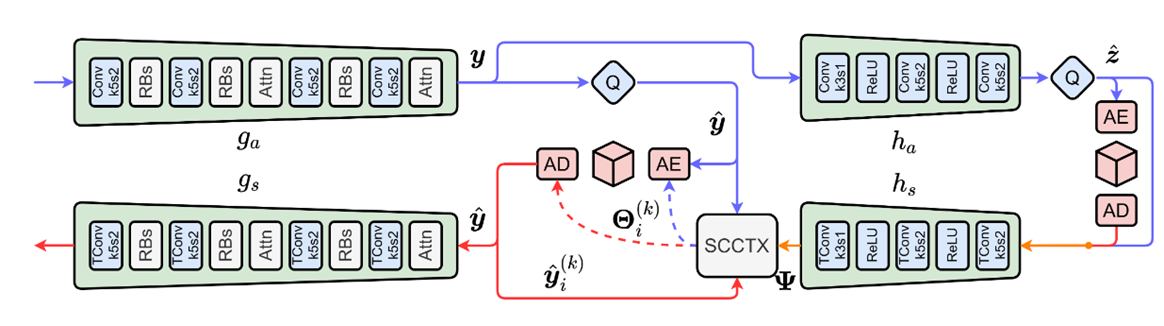
\includegraphics[width=3in]{architecture.png}
    \caption{Architecture of full ELIC \cite{ELIC}. The
blue and red arrows denote the encoding and decoding data flow. The orange ones are shared by both encoding and decoding. MAKE THE FIGURE AND CAPTION TO SPAN 2 COLUMNS}
    \label{fig:architecture}
\end{figure}

\begin{center}
\caption{Table \ref{table:architecture}: Architecture of ELIC-sm main transform networks. \cite{ELIC}}\\
\begin{tabular}{l|l}
\hline
Analyzer $g_a$ & Synthesizer $g_s$ \\
\hline
in: 3-channel image & in: M-channel symbols \\
\hline
Conv 5 $\times$ 5, s2, N & TConv 5 $\times$ 5, s2, N \\
ResBottleneck$\times$1 & ResBottleneck$\times$1 \\
Conv 5 $\times$ 5, s2, N & TConv 5 $\times$ 5, s2, N \\
ResBottleneck$\times$1 & ResBottleneck$\times$1 \\
Conv 5 $\times$ 5, s2, N & TConv 5 $\times$ 5, s2, N \\
ResBottleneck$\times$1 & ResBottleneck$\times$1 \\
Conv 5 $\times$ 5, s2, M & TConv 5 $\times$ 5, s2, 3 \\
\hline
\end{tabular}
\label{table:architecture}
\end{center}

We chose the smaller ELIC-sm architecture to reduce the amount of computational complexity and the need for data. We also kept the hyperparameters $M$ and $N$ reasonably low to further ease the training of the model. $M$ controls the number of channels in latent space and $N$ the number of channels in main transform networks. We leverage the ready-made implementation of Gaussian and arithmetic en/de-coders from CompressAI library \cite{compressai}. 

\subsection{Space-Channel Context model}
In works previously that ELIC \cite{ELIC} the context models were used only to predict either parameters of channel wise or spatial context to encode/decode pixels \cite{balle2016, mbt2018, balle2018, checkerboard}. The proposed method in ELIC uses both channel and spatial information in context model to predict the parameters $\mathbf{\Theta_i^{(k)}}$of next group \cite{ELIC}. 

The channel groups are formed in uneven manner based on observation that most of the energy is often concentrated on early channels. Therefore, the number of channels in groups is rising towards latter groups. The context prediction is made using all previous channel groups combined. When encoding or decoding the first channel group the channel wise context is therefore set to zeros. Because the uneven groups the sizes of inputs and outputs of the channel context model changes over the groups, and therefore separate model is implemented for each group. The number of networks is one less than number of groups because the networks make prediction of the next group parameters. The architecture of channel-wise context model is implemented as it is from the ELIC paper. \cite{ELIC} We doubled the number of channels only in the last convolutional layer.

The spatial context can be implemented as autoregressive convolution where each pixel prior to the current pixel must be predicted \cite{mbt2018}. A more efficient approach to implement spatial context prediction as checkerboard convolution introduced by He \textit{et al.} 2021 \cite{checkerboard}. The concept involves dividing the group into half like picking only the white or black squares from checkerboard and making predictions to these anchor pixels first. Another half of the group, the non-anchors, can be then predicted using the firstly encoded/decoded group as context. In the prediction of anchor parameters, the spatial context is simply set to zeros. The architecture of spatial context module is implemented with one checkerboard convolution layer with kernel size of 5 and stride of 1 that keeps the number of channels the same. 

The combined representation of prediction parameters is got from parameter aggregation network that combines the spatial and channel wise context predictions with hyperprior $\mathbf{\Psi}$ from hyperparameter synthetization network $h_s$. Because of uneven sizes of channel groups, channel and spatial context prediction networks, a separate networks needs to be implemented for each group. Architecture of parameter aggregation network is implemented as it is in the ELIC paper figure 6 with linear reduction of channels in layers \cite{ELIC}. 

The table \ref{table:SCCTX} shows the number of trainable parameters in thousands of SCCTX for channel number of $M=192$ and the default channel block sizes $(16,16,32,64,M-128)$ from the ELIC paper. The channel context model parameters for block$_0$ is \textit{NaN}, because it does not exists due to reasons discussed earlier. 

\begin{center}
\caption{Table \ref{table:SCCTX}: Number of trainable parameters in SCCTX in\\ thousands for each block ($b_i$) and for each component.}\\
\begin{tabular}{c c c c c c c} 
 \hline
 _ & b_0 & b_1 & b_2 & b_3 & b_4 & sum \\  
 \hline\hline
 channel & \textit{NaN} & 26 & 103 & 410 & 512 & 1050 \\
 \hline
 spatial & 13 & 13 & 51 & 205 & 205 & 487 \\
 \hline
 par.agg. & 198 & 198 & 277 & 480 & 480 & 1632 \\
 \hline
 sum & 210 & 236 & 431 & 1095 & 1197 & 3169 \\
 \hline
\end{tabular}
\label{table:SCCTX}
\end{center}

\subsection{Training versus compression flow}
The inference and training procedures differ from each other due to the undifferentiable nature of encoders. In inference time we want to compress the image to actual discrete bitstream and in training we want to just get the likelihoods from the entropy models and retain the gradient information. The gradient can be retained from the encoders by not compressing the image to bitstream, but just adding gaussian noise to image to mimic the effect of quantization. The approach was presented by \cite{balle2016}. 
With the checkerboard spatial context model another shortcut can be made in training time to further reduce the computational complexity of training. Following the work of He \textit{et al.} 2021 \cite{checkerboard} we used one pass encoding in training where parameters of non-anchor blocks are calculated from the input without calculating the parameters of anchor blocks. This approach was different from that presented in ELIC paper \cite{ELIC}, where they encoded $y+mu$ to bitstream instead of $y$ and therefore one pass encoding was not possible. We did not follow the implementation of ELIC because of lack of understanding about entropy models.

At inference time we calculate a separate bitstream to each image in batch sequentially and leverage the full context prediction by first decoding the anchor blocks and then the non-anchor blocks. This still allows us to decode the channel blocks in the image separately using the features of entropy model. However, for practical use cases, the batch processing should be allowed to benefit from the parallel computation capabilities of GPUs.

\section{Experiments}
\label{sec:experiments}
\subsection{Training} % Juha
\label{sec:training}

Training of the model was done with 6000 largest images from ImageNet \cite{imagenet} which were randomly cropped into size of 16x16 pixels.
These images were then run through the forward method of the network.
The forward method of the network does not fully compress the images but it transforms them into the latent spaces and the loss function takes into account the likelihood of good compression ratio as well as mse loss.

The model was trained with multiple different configurations. We tried $\lambda \in \{0.0008, 0,001\}$ where latent space channels $M$ and $N$ were $M=N=192$ and $\lambda \in \{0.0004, 0.0008\}$ where latent space channels $M$ and $N$ were $M=192, N=128$.
All of these models were trained for approximately 300 epochs but they could be still trained further.
Unfortunately due to lack of computational capabilities we could not train more networks and even these networks most likely could have been trained for longer but with epochs taking from 180 seconds (for smaller latent space) to 300 seconds (larger latent space), we could not train them further due to time constraints.



\vfill\pagebreak
\vfill\pagebreak

\section{Formatting your paper}
\label{sec:format}

All printed material, including text, illustrations, and charts, must be kept
within a print area of 7 inches (178 mm) wide by 9 inches (229 mm) high. Do
not write or print anything outside the print area. The top margin must be 1
inch (25 mm), except for the title page, and the left margin must be 0.75 inch
(19 mm).  All {\it text} must be in a two-column format. Columns are to be 3.39
inches (86 mm) wide, with a 0.24 inch (6 mm) space between them. Text must be
fully justified.

\section{PAGE TITLE SECTION}
\label{sec:pagestyle}

The paper title (on the first page) should begin 1.38 inches (35 mm) from the
top edge of the page, centered, completely capitalized, and in Times 14-point,
boldface type.  The authors' name(s) and affiliation(s) appear below the title
in capital and lower case letters.  Papers with multiple authors and
affiliations may require two or more lines for this information. Please note
that papers should not be submitted blind; include the authors' names on the
PDF.

\section{TYPE-STYLE AND FONTS}
\label{sec:typestyle}

To achieve the best rendering both in printed proceedings and electronic proceedings, we
strongly encourage you to use Times-Roman font.  In addition, this will give
the proceedings a more uniform look.  Use a font that is no smaller than nine
point type throughout the paper, including figure captions.

In nine point type font, capital letters are 2 mm high.  {\bf If you use the
smallest point size, there should be no more than 3.2 lines/cm (8 lines/inch)
vertically.}  This is a minimum spacing; 2.75 lines/cm (7 lines/inch) will make
the paper much more readable.  Larger type sizes require correspondingly larger
vertical spacing.  Please do not double-space your paper.  TrueType or
Postscript Type 1 fonts are preferred.

The first paragraph in each section should not be indented, but all the
following paragraphs within the section should be indented as these paragraphs
demonstrate.

\section{MAJOR HEADINGS}
\label{sec:majhead}

Major headings, for example, "1. Introduction", should appear in all capital
letters, bold face if possible, centered in the column, with one blank line
before, and one blank line after. Use a period (".") after the heading number,
not a colon.

\subsection{Subheadings}
\label{ssec:subhead}

Subheadings should appear in lower case (initial word capitalized) in
boldface.  They should start at the left margin on a separate line.
 
\subsubsection{Sub-subheadings}
\label{sssec:subsubhead}

Sub-subheadings, as in this paragraph, are discouraged. However, if you
must use them, they should appear in lower case (initial word
capitalized) and start at the left margin on a separate line, with paragraph
text beginning on the following line.  They should be in italics.

\section{PRINTING YOUR PAPER}
\label{sec:print}

Print your properly formatted text on high-quality, 8.5 x 11-inch white printer
paper. A4 paper is also acceptable, but please leave the extra 0.5 inch (12 mm)
empty at the BOTTOM of the page and follow the top and left margins as
specified.  If the last page of your paper is only partially filled, arrange
the columns so that they are evenly balanced if possible, rather than having
one long column.

In LaTeX, to start a new column (but not a new page) and help balance the
last-page column lengths, you can use the command ``$\backslash$pagebreak'' as
demonstrated on this page (see the LaTeX source below).

\section{PAGE NUMBERING}
\label{sec:page}

Please do {\bf not} paginate your paper.  Page numbers, session numbers, and
conference identification will be inserted when the paper is included in the
proceedings.

\section{ILLUSTRATIONS, GRAPHS, AND PHOTOGRAPHS}
\label{sec:illust}

Illustrations must appear within the designated margins.  They may span the two
columns.  If possible, position illustrations at the top of columns, rather
than in the middle or at the bottom.  Caption and number every illustration.
All halftone illustrations must be clear black and white prints.  Colors may be
used, but they should be selected so as to be readable when printed on a
black-only printer.

Since there are many ways, often incompatible, of including images (e.g., with
experimental results) in a LaTeX document, below is an example of how to do
this \cite{Lamp86}.

\section{FOOTNOTES}
\label{sec:foot}

Use footnotes sparingly (or not at all!) and place them at the bottom of the
column on the page on which they are referenced. Use Times 9-point type,
single-spaced. To help your readers, avoid using footnotes altogether and
include necessary peripheral observations in the text (within parentheses, if
you prefer, as in this sentence).

% Below is an example of how to insert images. Delete the ``\vspace'' line,
% uncomment the preceding line ``\centerline...'' and replace ``imageX.ps''
% with a suitable PostScript file name.
% -------------------------------------------------------------------------
\begin{figure}[htb]

\begin{minipage}[b]{1.0\linewidth}
  \centering
  \centerline{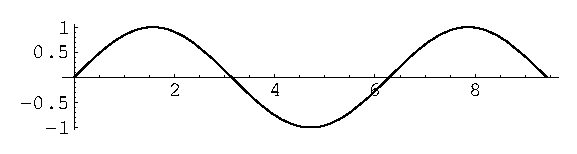
\includegraphics[width=8.5cm]{image1}}
%  \vspace{2.0cm}
  \centerline{(a) Result 1}\medskip
\end{minipage}
%
\begin{minipage}[b]{.48\linewidth}
  \centering
  \centerline{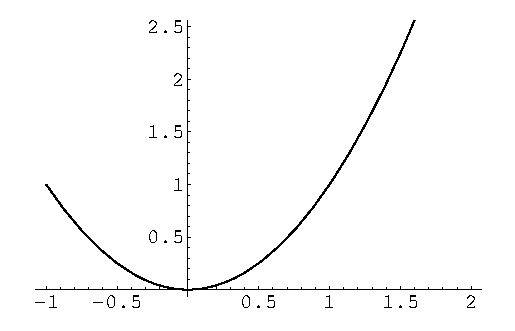
\includegraphics[width=4.0cm]{image3}}
%  \vspace{1.5cm}
  \centerline{(b) Results 3}\medskip
\end{minipage}
\hfill
\begin{minipage}[b]{0.48\linewidth}
  \centering
  \centerline{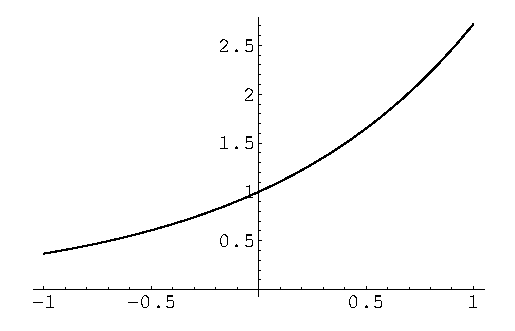
\includegraphics[width=4.0cm]{image4}}
%  \vspace{1.5cm}
  \centerline{(c) Result 4}\medskip
\end{minipage}
%
\caption{Example of placing a figure with experimental results.}
\label{fig:res}
%
\end{figure}


% To start a new column (but not a new page) and help balance the last-page
% column length use \vfill\pagebreak.
% -------------------------------------------------------------------------
%\vfill
%\pagebreak

\section{COPYRIGHT FORMS}
\label{sec:copyright}

You must submit your fully completed, signed IEEE electronic copyright release
form when you submit your paper. We {\bf must} have this form before your paper
can be published in the proceedings.

\section{RELATION TO PRIOR WORK}
\label{sec:prior}

The text of the paper should contain discussions on how the paper's
contributions are related to prior work in the field. It is important
to put new work in  context, to give credit to foundational work, and
to provide details associated with the previous work that have appeared
in the literature. This discussion may be a separate, numbered section
or it may appear elsewhere in the body of the manuscript, but it must
be present.

You should differentiate what is new and how your work expands on
or takes a different path from the prior studies. An example might
read something to the effect: "The work presented here has focused
on the formulation of the ABC algorithm, which takes advantage of
non-uniform time-frequency domain analysis of data. The work by
Smith and Cohen \cite{Lamp86} considers only fixed time-domain analysis and
the work by Jones et al \cite{C2} takes a different approach based on
fixed frequency partitioning. While the present study is related
to recent approaches in time-frequency analysis [3-5], it capitalizes
on a new feature space, which was not considered in these earlier
studies."

\vfill\pagebreak

\section{REFERENCES}
\label{sec:refs}

List and number all bibliographical references at the end of the
paper. The references can be numbered in alphabetic order or in
order of appearance in the document. When referring to them in
the text, type the corresponding reference number in square
brackets as shown at the end of this sentence \cite{C2}. An
additional final page (the fifth page, in most cases) is
allowed, but must contain only references to the prior
literature.

% References should be produced using the bibtex program from suitable
% BiBTeX files (here: strings, refs, manuals). The IEEEbib.bst bibliography
% style file from IEEE produces unsorted bibliography list.
% -------------------------------------------------------------------------
\bibliographystyle{IEEEbib}
\bibliography{strings,refs}

\end{document}
